\documentclass[a4paper,10pt]{article}
%\documentclass[a4paper,10pt]{scrartcl}

\usepackage[utf8]{inputenc}
  \usepackage[utf8]{inputenc}
  \usepackage[T1]{fontenc}
  \usepackage{lmodern}
  \usepackage{eso-pic}
  \usepackage{transparent}
  \usepackage{graphicx}
  \usepackage[colorlinks=true,linkcolor=black,urlcolor=black]{hyperref}
\newenvironment{figureH} {%
\begin{figure}[H]
}{%
\end{figure}
}
\title{}
\author{}
\date{}

\pdfinfo{%
  /Title    ()
  /Author   ()
  /Creator  ()
  /Producer ()
  /Subject  ()
  /Keywords ()
}

\begin{document}
\maketitle
  \begin{figureH}
        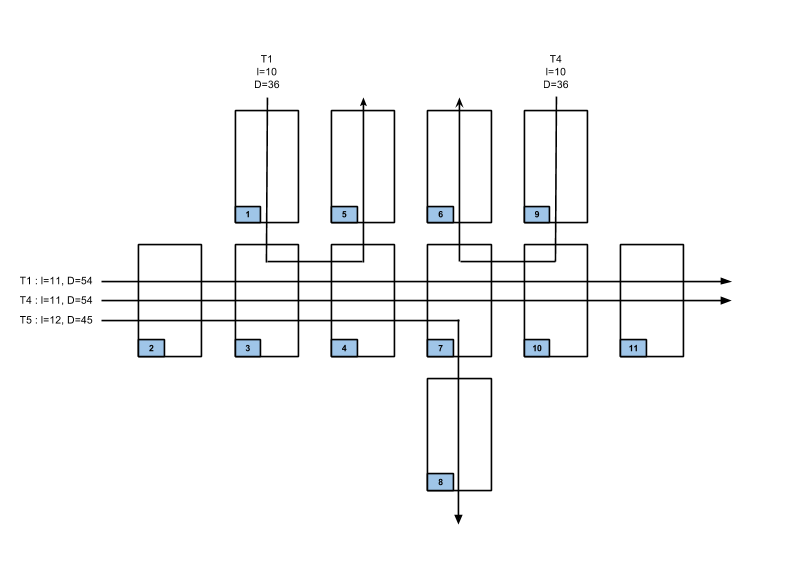
\includegraphics[width=\textwidth]{images/global.png}
        \center
        \caption{Schéma de l'example de la section 5}
        \label{image_global}
    \end{figureH}
    
      \begin{figureH}
        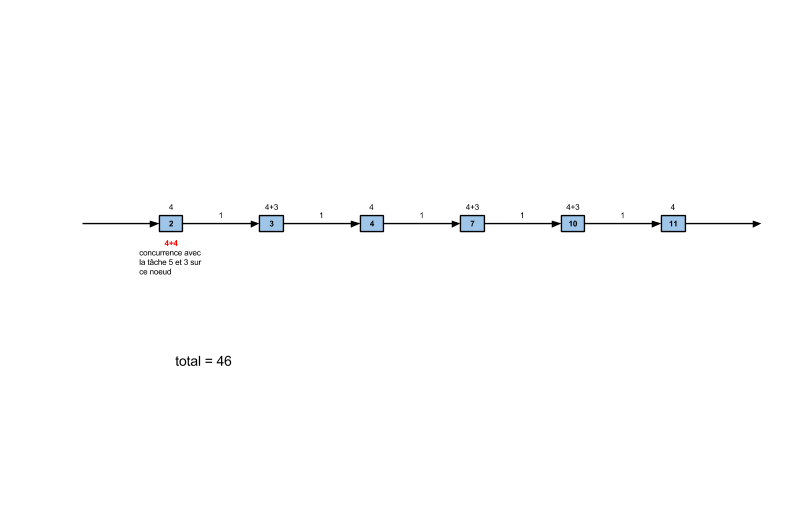
\includegraphics[width=\textwidth]{images/tache4.png}
        \center
        \caption{Chemin de la tache 4}
        \label{image_global}
    \end{figureH}
     \begin{figureH}
        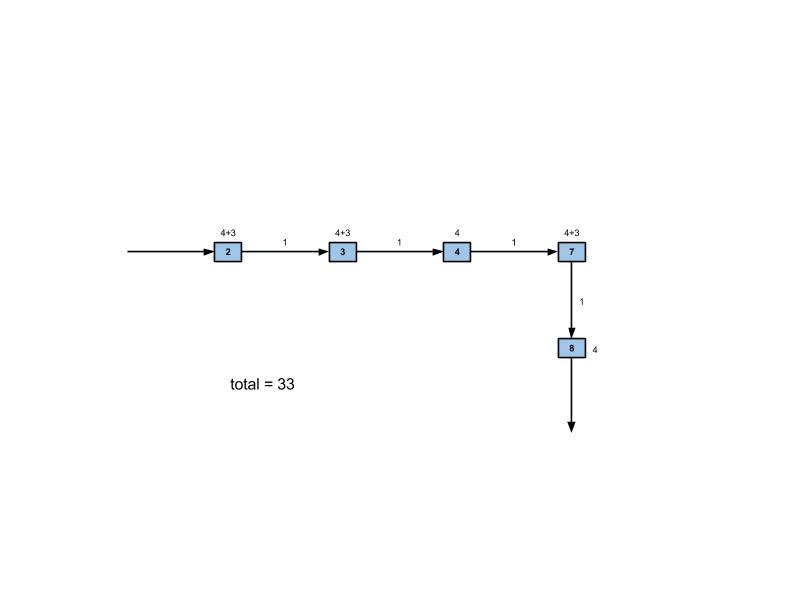
\includegraphics[width=\textwidth]{images/tache5.png}
        \center
        \caption{Chemin de la tache 5}
        \label{image_global}
    \end{figureH}
\end{document}
